%                                                                 aa.dem
% AA vers. 9.1, LaTeX class for Astronomy & Astrophysics
% demonstration file
%                                                       (c) EDP Sciences
%-----------------------------------------------------------------------
%
%\documentclass[referee]{aa} % for a referee version
%\documentclass[onecolumn]{aa} % for a paper on 1 column  
%\documentclass[longauth]{aa} % for the long lists of affiliations 
%\documentclass[letter]{aa} % for the letters 
%\documentclass[bibyear]{aa} % if the references are not structured 
%                              according to the author-year natbib style

%
% \documentclass[draft]{aa} 
\documentclass{aa}

%
\usepackage{graphicx}
%%%%%%%%%%%%%%%%%%%%%%%%%%%%%%%%%%%%%%%%
\usepackage{txfonts}
%%%%%%%%%%%%%%%%%%%%%%%%%%%%%%%%%%%%%%%%
%\usepackage[options]{hyperref}
% To add links in your PDF file, use the package "hyperref"
% with options according to your LaTeX or PDFLaTeX drivers.
%
\usepackage[]{hyperref}
\hypersetup{colorlinks=true, urlcolor=blue, citecolor=cyan, pdfborder={0 0 0}}

\begin{document} 


\title{A detailed analysis of the most distant catalogued open clusters}
\subtitle{Re-assessing fundamental parameters with Gaia EDR3 and \texttt{ASteCA}}

\author{G. I. Perren\inst{1}
      \and
      M. S. Pera\inst{1}
      \and
      H. Navone\inst{2}
      \and
      R. A. Vázquez\inst{3}
      % \fnmsep\thanks{Just to show the usage
      % of the elements in the author field}
}

\institute{Instituto de Astrof\'isica de La Plata (IALP-CONICET), La Plata,
Argentina\\
\email{gabrielperren@gmail.com}
\and
Facultad de Ciencias Exactas, Ingeniería y Agrimensura (UNR-IFIR-CONICET),
Rosario, Argentina
\and
Facultad de Ciencias Astronómicas y Geofísicas (UNLP-IALP-CONICET), 1900 La
Plata, Argentina
% \thanks{The university of heaven temporarily does not
%         accept e-mails}
}
\date{Received September 15, 2021; accepted December 16, 2021}

% \abstract{}{}{}{}{} 
% 5 {} token are mandatory
 
\abstract
% context heading (optional)
% {} leave it empty if necessary  
{Several studies have been presented in the last few years applying some kind of
automatic processing of data to estimate the fundamental parameters of open
clusters. These parameters are later on employed in larger scale analyses, for
example the structure of the Galaxy's spiral arms.
The distance is one of the more straightforward parameters to estimate, yet
enormous differences can still be found among published data. This is
particularly true for open clusters located more than a few Kpc away.}
% aims heading (mandatory)
{
We cross-matched several published catalogues and selected the twenty-five most
distant open clusters ($>$9000 Kpc). We then performed a detailed analysis of
their fundamental parameters, with emphasis on their distances, to determine the
agreement between catalogues and our estimates.}
% methods heading (mandatory)
{Photometric and astrometric data from the Gaia EDR3 survey was employed. The
data was processed with our own membership analysis code (pyUPMASK), and our
package for automatic fundamental cluster's parameters estimation
(\texttt{ASteCA}).}
% results heading (mandatory)
{We find differences in the estimated distances of up to several Kpc
between our results and those catalogued, even for the catalogues that show the
best matches with \texttt{ASteCA} values. Large differences are also found for
the age estimates.}
% conclusions heading (optional), leave it empty if necessary 
{Caution is thus strongly recommended when using catalogued parameters of open
clusters to infer large-scale properties of the Galaxy, particularly for those
located more than a few Kpc away.}

\keywords{
  Methods: statistical --
  Galaxies: star clusters: general --
  (Galaxy:) open clusters and associations: general --
  Techniques: photometric--
  Parallaxes --
  Proper motions
}

\maketitle


\section{Introduction}

 Open clusters (OCs) are not only used as laboratories to investigate stellar
 evolution, they are also routinely employed in the analysis of the Milky Way's
 structure~\citep{Loktin_1992,Moitinho_2006,Vazquez2008,Moitinho_2010}.
 Young OCs for example are known to be particularly
 useful in the tracing of spiral arms, as they have not yet drifted too far
 from their birth position~\citep{carraro_2013,Molina_2018}. As deeper, more
 complete, and more precise photometric and astrometric data becomes available,
 these studies will inevitably be extended towards more distant regions of the
 Galaxy.\\

 \textbf{AGREGARCONTENIDO ACA}\\

 This article is structured as follows. In Sect~\ref{sec:cat_clust_data} we
 introduce the stellar cluster catalogues, the clusters selected to be
 analyzed (crossed-matched from those catalogues), and the photometric and 
 astrometric data used to perform the analysis. Sect~\ref{sec:clust_analy}
 presents the methods employed in the study of all the clusters. The comparison
 of the estimated parameters with the catalogued values for each cluster is done
 in Sect~\ref{sec:results}. Finally, conclusions are highlighted in
 Sect~\ref{sec:conclusions}.





% =============================================================================
\section{Catalogues, clusters, and data}
 \label{sec:cat_clust_data}

 We chose four catalogues to cross-match and subsequently select the most
 distant clusters: \citet[][New Catalog of Optically Visible Open Clusters and
 Candidates, hereinafter OC]{Dias_2002},~\citet[][WEBDA,\footnote{
 \url{https://webda.physics.muni.cz/}} hereinafter WB]{Netopil_2012},
 \citet[][Milky Way Star Clusters Catalog, hereinafter MW]{Kharchenko_2012},
 and~\citet[][hereinafter CG]{Cantat_2020}.
 %
 The first two (OC and WB) are compilations of open clusters' fundamental
 parameters from the literature. They contain around 1700 (WB) and 2100 
 (OC) entries, and are heavily used in the field of open cluster research.
 The parameter values in both catalogues are heterogeneous, being compiled from
 various sources.
 The MW catalog is the largest one ($\sim$3000 entries) and, similarly to the CG
 catalog ($\sim$2000 entries), is composed of homogeneous fundamental parameter
 values obtained for all its entries. The method employed by the authors of the
 MW catalog is a semi-automated isochrone fit, while the CG catalog was
 generated employing an artificial neural network (trained on parameter values
 taken from the literature).

 Since we are interested in the open clusters most distant from the Sun, we
 select from these cross-matched catalogues those that are located at a
 distance of 9 Kpc or more in either of them. This is an arbitrary value that
 results in enough clusters to draw general conclusions, but not too many that
 would impede their detailed analysis.
 The initial full list consisted of thirty-eight open clusters. Eleven of these
 were found only in the MW catalog with distances larger than 9000 pc. These are
 either listed with substantially smaller distances in the other catalogs, or
 too sparse and or dubious. Hence these clusters were removed from the
 cross-matched list.
 %
 Two other clusters were also removed: Shorlin 1 ($\alpha_{2000}$=166.44,
 $\delta_{2000}$=-61.23) and FSR0338
 ($\alpha_{2000}$=327.93, $\delta_{2000}$=55.33). The latter appears in WB and
 MW at a distance of 12600 pc and 5600 pc respectively, while the former is
 listed only in MW with a distance of 14655 pc. Shorlin1 is studied
 in~\cite{Carraro_2009} and~\cite{Turner_2012}; in both cases the authors
 conclude that this is not a real cluster but a grouping of young stars.
 % Shorlin 1
 %
 % Carraro & Costa (2009)
 % > We also present evidence that this extremely distant group, formerly assumed
 % to be a star cluster (Shorlin 1), is a diffuse, young population, typically
 % found in spiral galaxies.
 %
 % Turner (2012)
 % > ...star counts also imply that Shorlin 1 is unlikely to represent a true
 % cluster, but is instead merely the trapezium-like remains of a previously-
 % bound cluster with an implied age of only a few Myr, according to the likely
 % presence of O-type stars within its boundaries.
 %
 FSR0338 is analyzed in~\cite{Froebrich_2010} where a distance of 6000 pc is
 assigned, but with large uncertainties.
 % Froebrich et al. (2010)
 % > Th high probability members of this newly identified cluster seem to indicate
 % an object with an age of 0.4 Gyrs at a distance of 6 kpc. The scatter in the
 % data points suggests larger than normal uncertainties for the parameters.
 %
 In both cases we find no evidence of a true stellar cluster in these regions.
 We base our conclusion on two findings. First, the large proper motions
 dispersion of the stars that occupy the overdensity around the central
 coordinates assigned to either object. Second, the lack of a clear sequence in
 their respective color-magnitude diagrams (CMD). These two clusters are thus
 discarded from further analysis. The remaining twenty-five clusters that will
 be studied in this work are shown in Table~\ref{tab:clusters}. Most of the
 selected clusters are located in the Third Quadrant with all of them in the
 latitude range of [-12$^{\circ}$, 8$^{\circ}$], relatively close to the
 galactic plane.

 \begin{table*}
 \caption{Selected catalogued open clusters with a distance $\geq$9000 pc,
 ordered by right ascension. The ages are expressed as the logarithm, and the
 distances are in parsec. In parenthesis, the short names used for the clusters
 throughout the article.}
 \label{tab:clusters}
 \centering
 % \begin{tabular}{lcccccccccc}
 \begin{tabular}{lllllllllll}
 \hline\hline
 Cluster & $\alpha_{2000}$  & $\delta_{2000}$ & OC$_{age}$ & OC$_{dist}$ & CG$_{age}$ &
 CG$_{dist}$ & WB$_{age}$ & WB$_{dist}$ & MW$_{age}$ & MW$_{dist}$ \\
 \hline
 Berkeley 73 (BER73)     & 95.5   & -6.35     & 9.18  & 9800  & 9.15  & 6158  &
 9.36 & 6850 & 9.15  & 7881  \\
 Berkeley 25 (BER25)     & 100.25 & -16.52    & 9.7   & 11400 & 9.39  & 6780  &
 9.6   & 11300 &  9.7   & 11400 \\
 Berkeley  75 (BER75)     & 102.25 & -24       & 9.6   & 9100  & 9.23  &  8304 
 & 9.48  & 9800  & 9.3   & 6273  \\
 Berkeley  26 (BER26)     & 102.58 & 5.75      & 9.6   & 12589 & -   & -   & 9.6
 & 4300  & 8.71  & 2724  \\
 Berkeley  29 (BER29)     & 103.27 & 16.93     & 9.025 & 14871 & 9.49  & 12604 &
 9.025 & 14871 & 9.1   & 10797 \\
 Tombaugh 2 (TOMB2)     & 105.77 & -20.82    & 9.01  & 6080  & 9.21  & 9316  &
 9.01 & 13260 & 9.01  & 6565  \\
 Berkeley 76 (BER76)     & 106.67 & -11.73    & 9.18  & 12600 & 9.22  & 4746  &
 9.18 & 12600 & 8.87  & 2360  \\
 FSR 1212 (F1212)   & 106.94 & -14.15    & -   & -   & 9.14  & 9682  & -   & -
 & 8.65  & 1780  \\
 Saurer 1 (SAU1)   & 110.23 & 1.81      & 9.7   & 13200 & -   & -   & 9.85  &
 13200 & 9.6   & 13719 \\
 Czernik 30 (CZER30)    & 112.83 & -9.97     & 9.4   & 9120  & 9.46  & 6647  &
 9.4 & 6200  & 9.2   & 6812  \\
 Arp-Madore 2 (ARPM2)     & 114.69 & -33.84    & 9.335 & 13341 & 9.48  & 11751 &
 9.335 & 13341 & 9.335 & 13338 \\
 vd Bergh-Hagen 4 (BH4)     & 114.43 & -36.07    & -   & -   & -   & -  
 & 8.3   & 19300 & -   & -   \\
 FSR 1419 (F1419)   & 124.71 & -47.79    & -   & -   & 9.21  & 11165 & -   & -   & 8.375 & 7746  \\
 vd Bergh-Hagen 37 (BH37)    & 128.95 & -43.62    & 8.84  & 11220 & 8.24 
 & 4038  & 8.85  & 2500  & 7.5   & 5202  \\
 ESO 092 05 (E9205)  & 150.81 & -64.75    & 9.3   & 5168  & 9.65  & 12444 &
 9.78  & 10900 & 9.3   & 5168  \\
 ESO 092 18 (E9218)  & 153.74 & -64.61    & 9.024 & 10607 & 9.46  & 9910  &
 9.024 & 607   & 9.15  & 9548  \\
 Saurer 3 (SAU3)   & 160.35 & -55.31    & 9.3   & 9550  & -   & -   & 9.45  &
 8830 & 9.3   & 7075  \\
 Kronberger 39 (KRON39)    & 163.56 & -61.74    & -   & 11100 & -   & -   & -   &
 -   & 6     & 4372  \\
 ESO 093 08 (E9308)  & 169.92 & -65.22    & 9.74  & 14000 & -   & -   & 9.65  &
 3700  & 9.8   & 13797 \\
 vd Bergh-Hagen 144 (BH144)   & 198.78 & -65.92    & 8.9   & 12000 & 9.17
 & 9649  & 8.9   & 12000 & 9     & 7241  \\
 vd Bergh-Hagen 176 (BH176)   & 234.85 & -50.05    & -   & -   & -   & - 
 & -   & 13400 & 9.8   & 18887 \\
 Kronberger 31 (KRON31)    & 295.05 & 26.26     & -   & 11900 & -   & -   & -   &
 -   & 8.5   & 12617 \\
 Saurer 6 (SAU6)   & 297.76 & 32.24     & 9.29  & 9330  & -   & -   & 9.29  &
 9330 & 9.2   & 7329  \\
 Berkeley 56 (BER56)     & 319.43 & 41.83     & 9.6   & 12100 & 9.47  & 9516  &
 9.6 & 12100 & 9.4   & 13180 \\
 Berkeley 102 (BER102)    & 354.66 & 56.64     & 9.5   & 9638  & 9.59  & 10519 &
 8.78  & 2600  & 9.14  & 4900 \\
 \hline
 \end{tabular}
 \end{table*}

 There are two other major works where a large catalog of analyzed open clusters
 is presented: \cite{Lui_2019} and \cite{Dias_2021}. The latter does not contain
 clusters with such large distances, and was hence not used. The former lists
 only four, and their values will be included in the discussion of the results
 in Sect.~\ref{sec:results}.\\

 Data from Gaia EDR3~\citep{Gaia_2016,Gaia_EDR3} was retrieved for a box of 20
 arcmin of length around the central coordinates for all the clusters. A small
 synopsis for each cluster is presented below, in alphabetical order:\\

 \noindent\textbf{Arp-Madore 2}: Lorem ipsum dolor sit amet, consectetur adipiscing elit. Donec libero lorem, varius eget elementum a, scelerisque vitae massa. Cras at neque interdum, pellentesque ipsum a, varius erat. Fusce ut dui vel mi euismod consequat eget eget felis. Suspendisse blandit erat eu enim ultricies, sed porttitor dolor placerat. Sed et semper.\\

 \noindent\textbf{Berkeley 25}: Lorem ipsum dolor sit amet, consectetur adipiscing elit. Donec libero lorem, varius eget elementum a, scelerisque vitae massa. Cras at neque interdum, pellentesque ipsum a, varius erat. Fusce ut dui vel mi euismod consequat eget eget felis. Suspendisse blandit erat eu enim ultricies, sed porttitor dolor placerat. Sed et semper.\\

 \noindent\textbf{Berkeley 26}: Lorem ipsum dolor sit amet, consectetur adipiscing elit. Donec libero lorem, varius eget elementum a, scelerisque vitae massa. Cras at neque interdum, pellentesque ipsum a, varius erat. Fusce ut dui vel mi euismod consequat eget eget felis. Suspendisse blandit erat eu enim ultricies, sed porttitor dolor placerat. Sed et semper.\\

 \noindent\textbf{Berkeley 29}: Lorem ipsum dolor sit amet, consectetur adipiscing elit. Donec libero lorem, varius eget elementum a, scelerisque vitae massa. Cras at neque interdum, pellentesque ipsum a, varius erat. Fusce ut dui vel mi euismod consequat eget eget felis. Suspendisse blandit erat eu enim ultricies, sed porttitor dolor placerat. Sed et semper.\\

 \noindent\textbf{Berkeley 56}: Lorem ipsum dolor sit amet, consectetur adipiscing elit. Donec libero lorem, varius eget elementum a, scelerisque vitae massa. Cras at neque interdum, pellentesque ipsum a, varius erat. Fusce ut dui vel mi euismod consequat eget eget felis. Suspendisse blandit erat eu enim ultricies, sed porttitor dolor placerat. Sed et semper.\\

 \noindent\textbf{Berkeley 73}: Lorem ipsum dolor sit amet, consectetur adipiscing elit. Donec libero lorem, varius eget elementum a, scelerisque vitae massa. Cras at neque interdum, pellentesque ipsum a, varius erat. Fusce ut dui vel mi euismod consequat eget eget felis. Suspendisse blandit erat eu enim ultricies, sed porttitor dolor placerat. Sed et semper.\\

 \noindent\textbf{Berkeley 75}: Lorem ipsum dolor sit amet, consectetur adipiscing elit. Donec libero lorem, varius eget elementum a, scelerisque vitae massa. Cras at neque interdum, pellentesque ipsum a, varius erat. Fusce ut dui vel mi euismod consequat eget eget felis. Suspendisse blandit erat eu enim ultricies, sed porttitor dolor placerat. Sed et semper.\\

 \noindent\textbf{Berkeley 76}: Lorem ipsum dolor sit amet, consectetur adipiscing elit. Donec libero lorem, varius eget elementum a, scelerisque vitae massa. Cras at neque interdum, pellentesque ipsum a, varius erat. Fusce ut dui vel mi euismod consequat eget eget felis. Suspendisse blandit erat eu enim ultricies, sed porttitor dolor placerat. Sed et semper.\\

 \noindent\textbf{Berkeley 102}: Lorem ipsum dolor sit amet, consectetur adipiscing elit. Donec libero lorem, varius eget elementum a, scelerisque vitae massa. Cras at neque interdum, pellentesque ipsum a, varius erat. Fusce ut dui vel mi euismod consequat eget eget felis. Suspendisse blandit erat eu enim ultricies, sed porttitor dolor placerat. Sed et semper.\\

 \noindent\textbf{Czernik 30}: Lorem ipsum dolor sit amet, consectetur adipiscing elit. Donec libero lorem, varius eget elementum a, scelerisque vitae massa. Cras at neque interdum, pellentesque ipsum a, varius erat. Fusce ut dui vel mi euismod consequat eget eget felis. Suspendisse blandit erat eu enim ultricies, sed porttitor dolor placerat. Sed et semper.\\

 \noindent\textbf{ESO 092 05}: Lorem ipsum dolor sit amet, consectetur adipiscing elit. Donec libero lorem, varius eget elementum a, scelerisque vitae massa. Cras at neque interdum, pellentesque ipsum a, varius erat. Fusce ut dui vel mi euismod consequat eget eget felis. Suspendisse blandit erat eu enim ultricies, sed porttitor dolor placerat. Sed et semper.\\

 \noindent\textbf{ESO 092 18}: Lorem ipsum dolor sit amet, consectetur adipiscing elit. Donec libero lorem, varius eget elementum a, scelerisque vitae massa. Cras at neque interdum, pellentesque ipsum a, varius erat. Fusce ut dui vel mi euismod consequat eget eget felis. Suspendisse blandit erat eu enim ultricies, sed porttitor dolor placerat. Sed et semper.\\

 \noindent\textbf{ESO 093 08}: Lorem ipsum dolor sit amet, consectetur adipiscing elit. Donec libero lorem, varius eget elementum a, scelerisque vitae massa. Cras at neque interdum, pellentesque ipsum a, varius erat. Fusce ut dui vel mi euismod consequat eget eget felis. Suspendisse blandit erat eu enim ultricies, sed porttitor dolor placerat. Sed et semper.\\

 \noindent\textbf{FSR 1212}: Lorem ipsum dolor sit amet, consectetur adipiscing elit. Donec libero lorem, varius eget elementum a, scelerisque vitae massa. Cras at neque interdum, pellentesque ipsum a, varius erat. Fusce ut dui vel mi euismod consequat eget eget felis. Suspendisse blandit erat eu enim ultricies, sed porttitor dolor placerat. Sed et semper.\\

 \noindent\textbf{FSR 1419}: Lorem ipsum dolor sit amet, consectetur adipiscing elit. Donec libero lorem, varius eget elementum a, scelerisque vitae massa. Cras at neque interdum, pellentesque ipsum a, varius erat. Fusce ut dui vel mi euismod consequat eget eget felis. Suspendisse blandit erat eu enim ultricies, sed porttitor dolor placerat. Sed et semper.\\

 \noindent\textbf{Kronberger31} and \textbf{Kronberger39}: these two clusters
 where discovered and catalogued as \emph{Cluster candidates with RCs}
 in~\cite{Kronberger_2006}. Both show a very dispersed and scarcely populated
 sequence.\\

 \noindent\textbf{Saurer 1}: Lorem ipsum dolor sit amet, consectetur adipiscing elit. Donec libero lorem, varius eget elementum a, scelerisque vitae massa. Cras at neque interdum, pellentesque ipsum a, varius erat. Fusce ut dui vel mi euismod consequat eget eget felis. Suspendisse blandit erat eu enim ultricies, sed porttitor dolor placerat. Sed et semper.\\

 \noindent\textbf{Saurer 3}: Lorem ipsum dolor sit amet, consectetur adipiscing elit. Donec libero lorem, varius eget elementum a, scelerisque vitae massa. Cras at neque interdum, pellentesque ipsum a, varius erat. Fusce ut dui vel mi euismod consequat eget eget felis. Suspendisse blandit erat eu enim ultricies, sed porttitor dolor placerat. Sed et semper.\\

 \noindent\textbf{Saurer 6}: Lorem ipsum dolor sit amet, consectetur adipiscing elit. Donec libero lorem, varius eget elementum a, scelerisque vitae massa. Cras at neque interdum, pellentesque ipsum a, varius erat. Fusce ut dui vel mi euismod consequat eget eget felis. Suspendisse blandit erat eu enim ultricies, sed porttitor dolor placerat. Sed et semper.\\

 \noindent\textbf{Tombaugh 2}: Lorem ipsum dolor sit amet, consectetur adipiscing elit. Donec libero lorem, varius eget elementum a, scelerisque vitae massa. Cras at neque interdum, pellentesque ipsum a, varius erat. Fusce ut dui vel mi euismod consequat eget eget felis. Suspendisse blandit erat eu enim ultricies, sed porttitor dolor placerat. Sed et semper.\\

 \noindent\textbf{van den Bergh-Hagen 4}: Lorem ipsum dolor sit amet, consectetur adipiscing elit. Donec libero lorem, varius eget elementum a, scelerisque vitae massa. Cras at neque interdum, pellentesque ipsum a, varius erat. Fusce ut dui vel mi euismod consequat eget eget felis. Suspendisse blandit erat eu enim ultricies, sed porttitor dolor placerat. Sed et semper.\\

 \noindent\textbf{van den Bergh-Hagen 37}: Lorem ipsum dolor sit amet, consectetur adipiscing elit. Donec libero lorem, varius eget elementum a, scelerisque vitae massa. Cras at neque interdum, pellentesque ipsum a, varius erat. Fusce ut dui vel mi euismod consequat eget eget felis. Suspendisse blandit erat eu enim ultricies, sed porttitor dolor placerat. Sed et semper.\\

 \noindent\textbf{van den Bergh-Hagen 144}: Lorem ipsum dolor sit amet, consectetur adipiscing elit. Donec libero lorem, varius eget elementum a, scelerisque vitae massa. Cras at neque interdum, pellentesque ipsum a, varius erat. Fusce ut dui vel mi euismod consequat eget eget felis. Suspendisse blandit erat eu enim ultricies, sed porttitor dolor placerat. Sed et semper.\\

 \noindent\textbf{van den Bergh-Hagen 176}: Lorem ipsum dolor sit amet, consectetur adipiscing elit. Donec libero lorem, varius eget elementum a, scelerisque vitae massa. Cras at neque interdum, pellentesque ipsum a, varius erat. Fusce ut dui vel mi euismod consequat eget eget felis. Suspendisse blandit erat eu enim ultricies, sed porttitor dolor placerat. Sed et semper.\\


 In Fig~\ref{fig:MWmap} we show the twenty-five selected clusters for each of
 the four catalogues, positioned on the face-on view of the Galaxy The spiral
 arms are taken from~\cite{Momany_2006}. The large dispersion for the distances
 assigned to each cluster in different catalogs is clearly visible.

 \begin{figure*}
  \resizebox{\hsize}{!}{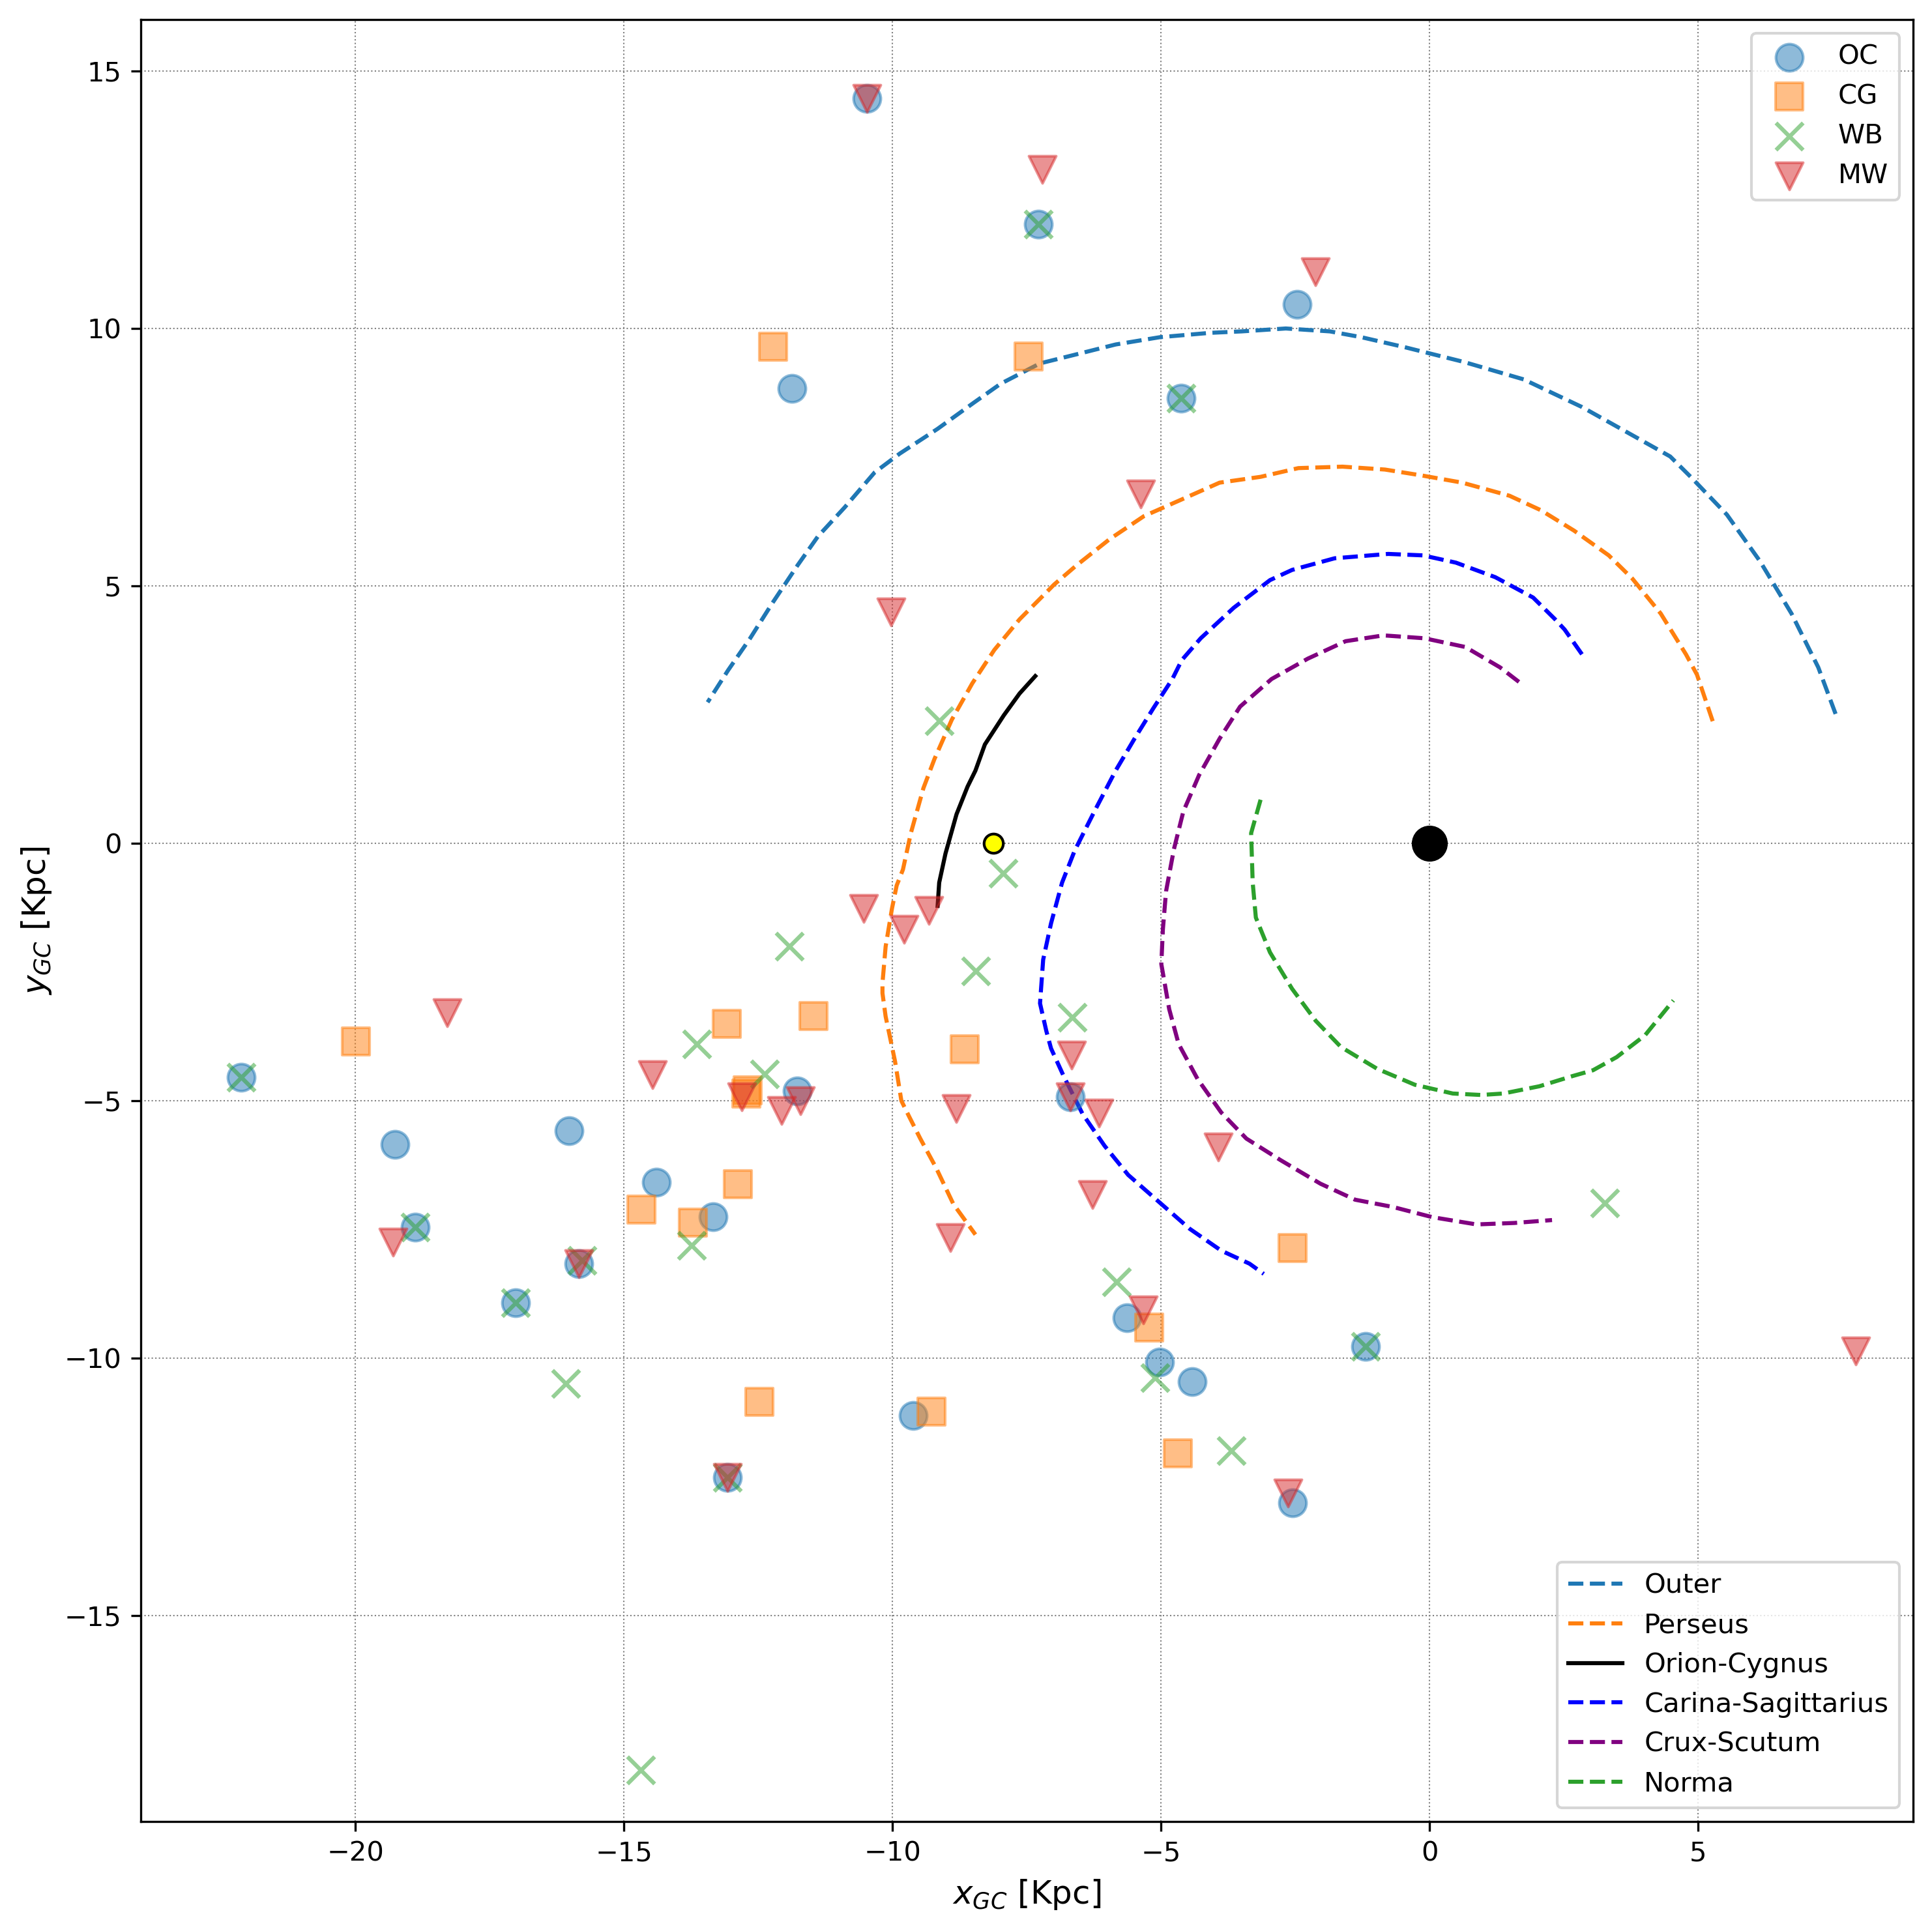
\includegraphics[]{figs/MWmap.png}}
  \caption{Position of the twenty-five clusters selected from the four catalogs
  mentioned in the text, on a face-on view of the Milky Way. The Sun and the
  center of the Galaxy are marked with a yellow filled circle and a black
  filled circle, respectively.}
  \label{fig:MWmap}
 \end{figure*}





% =============================================================================
\section{Cluster analysis}
 \label{sec:clust_analy}

 xxxxx





% =============================================================================
\section{Results}
 \label{sec:results}

 xxxxx





% =============================================================================
\section{Conclusions}
 \label{sec:conclusions}

 xxxxx




   %-------------------------------------- Two column figure (place early!)
   % \begin{figure*}
   % \centering
   % %%%\includegraphics{empty.eps}
   % %%%\includegraphics{empty.eps}
   % %%%\includegraphics{empty.eps}
   % \caption{Adiabatic exponent $\Gamma_1$.
   %             $\Gamma_1$ is plotted as a function of
   %             $\lg$ internal energy $\mathrm{[erg\,g^{-1}]}$ and $\lg$
   %             density $\mathrm{[g\,cm^{-3}]}$.}
   %            \label{FigGam}%
   %  \end{figure*}


   %--------------------------------------------------- One column table
%    \begin{table}
%       \caption[]{Opacity sources.}
%          \label{KapSou}
%      $$ 
%          \begin{array}{p{0.5\linewidth}l}
%             \hline
%             \noalign{\smallskip}
%             Source      &  T / {[\mathrm{K}]} \\
%             \noalign{\smallskip}
%             \hline
%             \noalign{\smallskip}
%             Yorke 1979, Yorke 1980a & \leq 1700^{\mathrm{a}}     \\
% %           Yorke 1979, Yorke 1980a & \leq 1700             \\
%             Kr\"ugel 1971           & 1700 \leq T \leq 5000 \\
%             Cox \& Stewart 1969     & 5000 \leq             \\
%             \noalign{\smallskip}
%             \hline
%          \end{array}
%      $$ 
%    \end{table}



%                                                One column figure
%----------------------------------------------------------------- 
% \begin{figure}
% \centering
% %%%\includegraphics[width=3cm]{empty.eps}
%    \caption{Vibrational stability equation of state
%             $S_{\mathrm{vib}}(\lg e, \lg \rho)$.
%             $>0$ means vibrational stability.
%            }
%       \label{FigVibStab}
% \end{figure}

\section{Conclusions}

xxx

\begin{acknowledgements}
This work has made use of data from the European Space Agency (ESA) mission
{\it Gaia} (\url{https://www.cosmos.esa.int/gaia}), processed by the {\it Gaia}
Data Processing and Analysis Consortium (DPAC,
\url{https://www.cosmos.esa.int/web/gaia/dpac/consortium}). Funding for the DPAC
has been provided by national institutions, in particular the institutions
participating in the {\it Gaia} Multilateral Agreement.
%
This research has made use of the WEBDA database, operated at the Department of
Theoretical Physics and Astrophysics of the Masaryk University.
%
This research has made use of the VizieR catalog access tool, operated at CDS,
Strasbourg, France~\citep{Ochsenbein_2000}.
%
This research has made use of ``Aladin sky atlas'' developed at
CDS, Strasbourg Observatory, France~\citep{Bonnarel2000,Boch2014}.
%
This research has made use of NASA's Astrophysics Data System.
%
This research made use of the Python language v3.7.3~\citep{vanRossum_1995}
and the following packages:
NumPy\footnote{\url{http://www.numpy.org/}}~\citep{vanDerWalt_2011};
SciPy\footnote{\url{http://www.scipy.org/}}~\citep{Jones_2001};
Astropy\footnote{\url{http://www.astropy.org/}}, a community-developed core
Python package for Astronomy \citep{Astropy_2013};
matplotlib\footnote{\url{http://matplotlib.org/}}~\citep{hunter_2007}
\end{acknowledgements}




\bibliographystyle{aa}
\bibliography{biblio} % your references Yourfile.bib

\end{document}


